\section{The Two Approaches Everyone Was Using (And Why Neither Was Great)}

Before 2014 or so, if you wanted to do machine translation, you did not use neural networks at all.
You used what were called \textbf{statistical machine translation} systems --- enormous lookup tables of phrase translations, stitched together by hand-engineered rules and a prayer.
They worked, sort of, in the way that a phrase book works when you are lost in Tokyo: you can get directions to the train station, but you are not having a philosophical discussion.

Neural networks changed the game by \emph{learning} the mapping from input to output.
Instead of hand-crafting rules, you show the model millions of translated sentence pairs and let it figure out the patterns.
By 2017, neural approaches had overtaken statistical ones on every major benchmark.

But within the neural world, there were two competing philosophies for how to process sequences.

\subsection{RNNs: One Word at a Time}

A \textbf{recurrent neural network} reads a sequence the way you read a sentence: left to right, one word at a time.
After each word, it updates an internal summary --- a \emph{hidden state} --- that represents ``everything I have seen so far.''
By the time it reaches the period, that hidden state is supposed to be a compressed representation of the entire sentence.

\begin{figure}[htb]
\centering
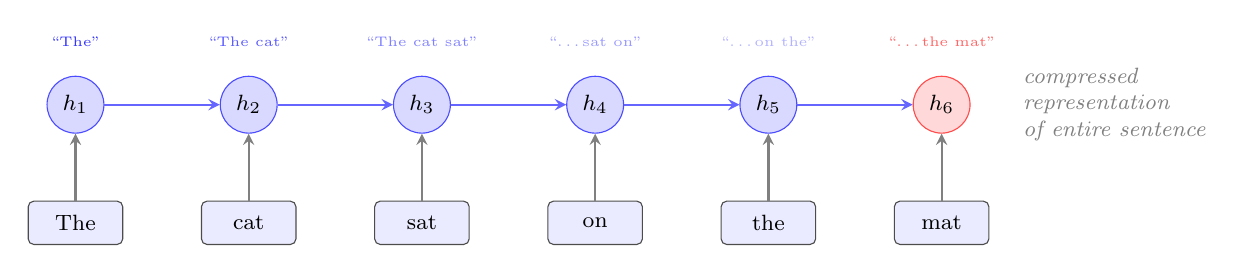
\begin{tikzpicture}[
    >=stealth,
    word/.style={rectangle, draw=black!70, fill=blue!8, rounded corners=2pt,
                 minimum width=1.2cm, minimum height=0.55cm, font=\footnotesize},
    state/.style={circle, draw=blue!70, fill=blue!15, minimum size=0.7cm,
                  font=\footnotesize\bfseries},
    final/.style={circle, draw=red!70, fill=red!15, minimum size=0.7cm,
                  font=\footnotesize\bfseries},
    arr/.style={->, thick, blue!60},
    feed/.style={->, thick, black!50},
]
  % Words
  \node[word] (w1) at (0, 0) {The};
  \node[word] (w2) at (2.2, 0) {cat};
  \node[word] (w3) at (4.4, 0) {sat};
  \node[word] (w4) at (6.6, 0) {on};
  \node[word] (w5) at (8.8, 0) {the};
  \node[word] (w6) at (11.0, 0) {mat};

  % Hidden states
  \node[state] (h1) at (0, 1.5) {$h_1$};
  \node[state] (h2) at (2.2, 1.5) {$h_2$};
  \node[state] (h3) at (4.4, 1.5) {$h_3$};
  \node[state] (h4) at (6.6, 1.5) {$h_4$};
  \node[state] (h5) at (8.8, 1.5) {$h_5$};
  \node[final] (h6) at (11.0, 1.5) {$h_6$};

  % Word -> hidden state arrows
  \foreach \i in {1,...,6} {
    \draw[feed] (w\i.north) -- (h\i.south);
  }

  % Hidden state chain
  \draw[arr] (h1) -- (h2);
  \draw[arr] (h2) -- (h3);
  \draw[arr] (h3) -- (h4);
  \draw[arr] (h4) -- (h5);
  \draw[arr] (h5) -- (h6);

  % Labels
  \node[font=\footnotesize\itshape, text=black!50, anchor=west] at (11.7, 1.5)
    {\begin{tabular}{l}compressed\\representation\\of entire sentence\end{tabular}};

  % Fade effect: progressively lighter info labels
  \node[font=\tiny, text=blue!80] at (0, 2.3) {``The''};
  \node[font=\tiny, text=blue!65] at (2.2, 2.3) {``The cat''};
  \node[font=\tiny, text=blue!50] at (4.4, 2.3) {``The cat sat''};
  \node[font=\tiny, text=blue!40] at (6.6, 2.3) {``\ldots sat on''};
  \node[font=\tiny, text=blue!30] at (8.8, 2.3) {``\ldots on the''};
  \node[font=\tiny, text=red!60] at (11.0, 2.3) {``\ldots the mat''};

\end{tikzpicture}
\caption{An RNN processes words sequentially, updating its hidden state at each step. Each $h_i$ represents the model's compressed understanding of everything up to word $i$. By $h_6$, the entire sentence must fit inside a single vector --- earlier words survive only to the extent they were not overwritten along the way.}
\end{figure}

The problem is that ``compressed'' is doing a lot of heavy lifting there.
Imagine playing a game of telephone with a hundred people.
Person 1 hears the original message.
Person 100 gets\ldots something.
Maybe it is related to the original.
Maybe not.

This is essentially the \textbf{vanishing gradient problem}: information from early in the sequence gets diluted as it passes through step after step.
People invented clever variants --- \textbf{LSTMs} and \textbf{GRUs} --- that add gating mechanisms to help the network decide what to remember and what to forget.
These helped a lot.
But they did not fix the deeper issue.

And there was another problem, arguably worse from an engineering standpoint: RNNs are \emph{sequential}.
You literally cannot process word 5 until you have finished with words 1 through 4.
In an era when GPUs were getting faster by putting thousands of cores in parallel, RNNs were the one architecture that could not take advantage of that.
It was like having a thousand-lane highway but only being allowed to send one car at a time.

\subsection{CNNs: Looking Through a Keyhole}

Convolutional neural networks come from the world of computer vision, where they are spectacularly successful.
The idea, adapted for sequences, is to look at small local windows of words --- say, three or five at a time --- and compute a summary of each window.
Then stack another layer on top, which looks at windows of those summaries, and so on.

The good news: each window is independent, so you \emph{can} parallelize.
A CNN does not have the one-car-at-a-time problem.

\begin{figure}[htb]
\centering
\begin{tikzpicture}[
    >=stealth,
    word/.style={rectangle, draw=black!70, fill=blue!8, rounded corners=2pt,
                 minimum width=1.1cm, minimum height=0.5cm, font=\footnotesize},
    summary/.style={rectangle, draw=green!70!black, fill=green!12, rounded corners=2pt,
                    minimum width=1.8cm, minimum height=0.5cm, font=\footnotesize},
    summary2/.style={rectangle, draw=orange!70!black, fill=orange!12, rounded corners=2pt,
                     minimum width=2.8cm, minimum height=0.5cm, font=\footnotesize},
    win/.style={draw=green!60!black, thick, rounded corners=3pt, dashed},
    win2/.style={draw=orange!60!black, thick, rounded corners=3pt, dashed},
    feed/.style={->, thick, black!40},
]
  % Layer 0: Words
  \def\sp{1.6}
  \node[word] (w1) at (0*\sp, 0) {The};
  \node[word] (w2) at (1*\sp, 0) {cat};
  \node[word] (w3) at (2*\sp, 0) {sat};
  \node[word] (w4) at (3*\sp, 0) {on};
  \node[word] (w5) at (4*\sp, 0) {the};
  \node[word] (w6) at (5*\sp, 0) {mat};

  \node[font=\footnotesize\itshape, text=black!50, anchor=east] at (-0.9, 0) {words};

  % Window brackets layer 1
  \node[win, fit=(w1)(w3), inner sep=4pt] (win1) {};
  \node[win, fit=(w2)(w4), inner sep=4pt] (win2) {};
  \node[win, fit=(w3)(w5), inner sep=4pt] (win3) {};
  \node[win, fit=(w4)(w6), inner sep=4pt] (win4) {};

  % Layer 1: Summaries
  \node[summary] (s1) at (1*\sp, 1.8) {$s_1$};
  \node[summary] (s2) at (2*\sp, 1.8) {$s_2$};
  \node[summary] (s3) at (3*\sp, 1.8) {$s_3$};
  \node[summary] (s4) at (4*\sp, 1.8) {$s_4$};

  \node[font=\footnotesize\itshape, text=black!50, anchor=east] at (-0.9, 1.8) {layer 1};

  % Arrows from windows to summaries
  \draw[feed] (0.5*\sp, 0.35) -- (s1.south west);
  \draw[feed] (1*\sp, 0.35) -- (s1.south);
  \draw[feed] (1.5*\sp, 0.35) -- (s1.south east);

  \draw[feed] (1.5*\sp, 0.35) -- (s2.south west);
  \draw[feed] (2*\sp, 0.35) -- (s2.south);
  \draw[feed] (2.5*\sp, 0.35) -- (s2.south east);

  \draw[feed] (2.5*\sp, 0.35) -- (s3.south west);
  \draw[feed] (3*\sp, 0.35) -- (s3.south);
  \draw[feed] (3.5*\sp, 0.35) -- (s3.south east);

  \draw[feed] (3.5*\sp, 0.35) -- (s4.south west);
  \draw[feed] (4*\sp, 0.35) -- (s4.south);
  \draw[feed] (4.5*\sp, 0.35) -- (s4.south east);

  % Window brackets layer 2
  \node[win2, fit=(s1)(s3), inner sep=4pt] {};
  \node[win2, fit=(s2)(s4), inner sep=4pt] {};

  % Layer 2: Higher summaries
  \node[summary2] (t1) at (2*\sp, 3.6) {$t_1$};
  \node[summary2] (t2) at (3*\sp, 3.6) {$t_2$};

  \node[font=\footnotesize\itshape, text=black!50, anchor=east] at (-0.9, 3.6) {layer 2};

  % Arrows layer 1 -> layer 2
  \draw[feed] (s1.north) -- (t1.south west);
  \draw[feed] (s2.north) -- (t1.south);
  \draw[feed] (s3.north) -- (t1.south east);

  \draw[feed] (s2.north) -- (t2.south west);
  \draw[feed] (s3.north) -- (t2.south);
  \draw[feed] (s4.north) -- (t2.south east);

  % Parallel annotation
  \draw[<->, thick, green!60!black] (0.2, -0.8) -- (5*\sp - 0.2, -0.8);
  \node[font=\footnotesize\itshape, text=green!50!black] at (2.5*\sp, -1.15) {all windows computed in parallel};

\end{tikzpicture}
\caption{A CNN for sequences. Layer~1 slides a window of three words across the input, computing a summary for each position --- all in parallel. Layer~2 does the same over layer~1's summaries, gradually building up longer-range understanding. To connect ``The'' and ``mat,'' you need enough layers for them to fall within the same window.}
\end{figure}

The bad news: if two words that depend on each other are far apart in the sentence, you need to stack a lot of layers before they fall within the same window.
It is like trying to understand a legal contract by only ever reading three consecutive words at a time.
You can build up to the big picture eventually, but it takes a while, and subtleties get lost.

By 2017, Facebook AI had a competitive CNN-based translation system called ConvS2S \cite{gehring2017convs2s} --- open-sourced as part of their \texttt{fairseq} toolkit\footnote{\url{https://github.com/facebookresearch/fairseq}} --- but the field had largely bet on RNNs --- specifically LSTMs --- as the default.
Both approaches had real limitations, and everyone knew it.
The question was whether there was a third option.
